\usetikzlibrary{patterns}
\pgfdeclareimage[width=3cm]{KawadaHRP3}{NMPCWalkgen/figures/HRP2-obstacle-avoidance-2.png}

\def\steppingstonefig{
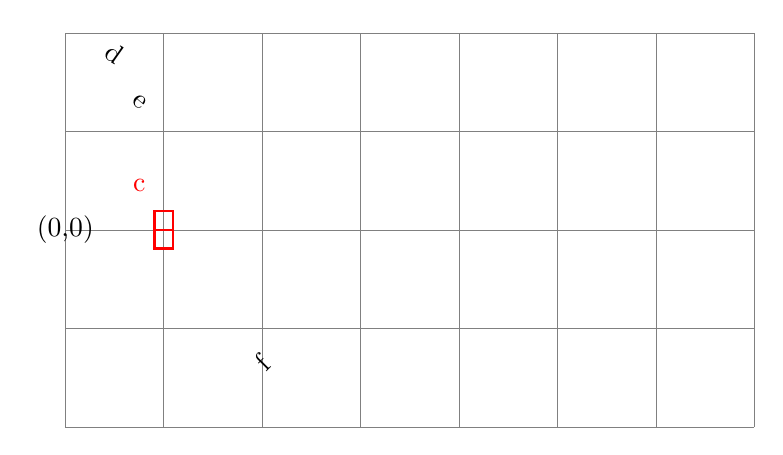
\begin{tikzpicture}[scale=1.25]
  \draw[help lines] (0,-2) grid (7,2);
             
  \path  (1.0, 0.095) node (a) [draw,color=red,thick] (1.2172,  0.233) {}
         (1.0,-0.095) node (b) [draw,color=red,thick] (1.2172, -0.233) {}
         (0.75, 0.45) node (c) [rectangle,color=red,thick] (1.25   , -0.45) {c}
         %
         (0.5 , 1.8)  node (d) [rectangle,color=black,thick,rotate=-35] (0.75   , 1.60) {d}
         (0.75, 1.3)  node (e) [rectangle,color=black,thick,rotate=-40] (1.0   ,  1.1)  {e}    
         %
         (2.0 , -1.35 ) node (f) [rectangle,color=black,thick,rotate=45] (2.5   ,-0.45) {f};   
  \node at (0,0) {(0,0)};
\end{tikzpicture}
}

\def\steppingstonefigtwo{
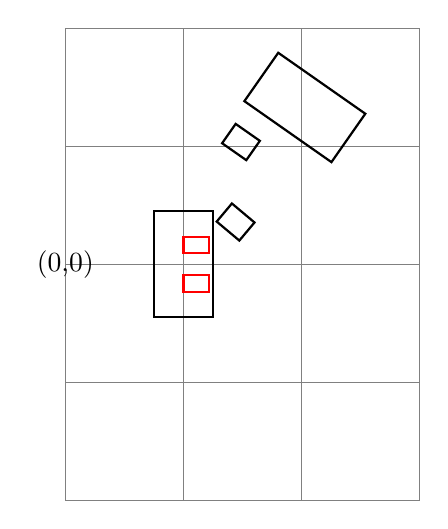
\begin{tikzpicture}[scale=1.5]
  \draw[help lines] (0,-2) grid (3,2);
             
  \draw[color=red  ,thick] (1.0, 0.095) rectangle (1.2172,  0.233);
  \draw[color=red,  thick] (1.0,-0.095) rectangle (1.2172, -0.233);

  \draw[color=black,thick] (0.75, 0.45) rectangle (1.25   , -0.45);

  \draw[color=black,thick,rotate=-35] (0.5 , 1.8) rectangle (0.75   , 1.60);
  \draw[color=black,thick,rotate=-40] (0.75, 1.3) rectangle (1.0   ,  1.1);       

  \draw[color=black,thick,rotate=55] (2.0 , -1.35 ) rectangle (2.5   ,-0.45);       
  \node at (0,0) {(0,0)};
\end{tikzpicture}
}

\def\problemtopology{
 \begin{pspicture}(-2,-2)(3,3)
  \psset{viewpoint=100 30 20,Decran=100}
  \psSolid[object=cube,a=2,
  action=draw*,
   fillcolor=magenta!20]
   \axesIIID[showOrigin=false,axisnames={x,y,\theta}](1,1,1)(3,2,2.5)
 \end{pspicture}
}
